
%(BEGIN_QUESTION)
% Copyright 2009, Tony R. Kuphaldt, released under the Creative Commons Attribution License (v 1.0)
% This means you may do almost anything with this work of mine, so long as you give me proper credit

This paint mixing system blends a ratio of clear base to colored pigment in order to produce a paint of the desired color.  A color analyzer senses how dark the mixed paint is, producing a 4-20 mA signal varying with color (4 mA = clear ; 20 mA = dark):
 
$$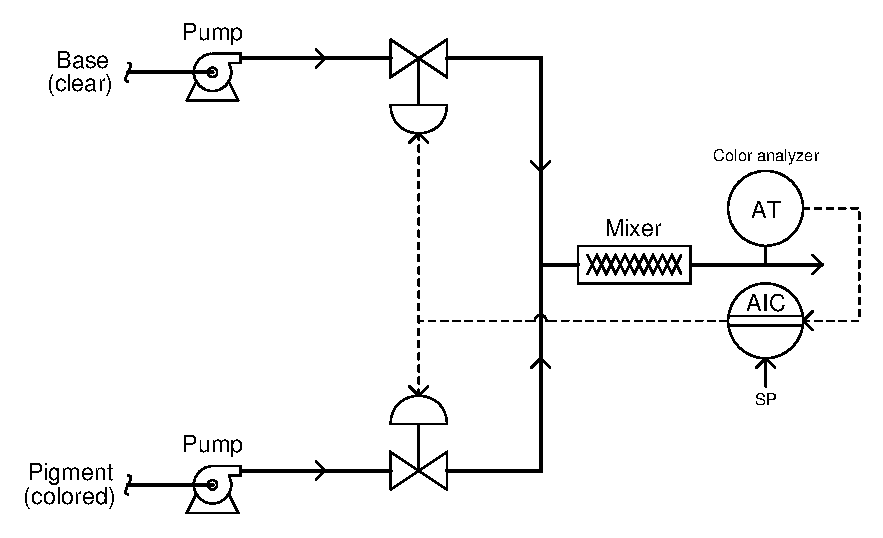
\includegraphics[width=15.5cm]{i03781x01.eps}$$

Assuming reverse action in the controller, determine the proper split ranges of the two control valves:

% No blank lines allowed between lines of an \halign structure!
% I use comments (%) instead, so that TeX doesn't choke.

$$\vbox{\offinterlineskip
\halign{\strut
\vrule \quad\hfil # \ \hfil & 
\vrule \quad\hfil # \ \hfil \vrule \cr
\noalign{\hrule}
%
% First row
Base valve position & Controller output signal \cr
%
\noalign{\hrule}
%
% Another row
Fully shut (0\%) & ??? mA \cr
%
\noalign{\hrule}
%
% Another row
Wide open (100\%) & ??? mA \cr
%
\noalign{\hrule}
} % End of \halign 
}$$ % End of \vbox

% No blank lines allowed between lines of an \halign structure!
% I use comments (%) instead, so that TeX doesn't choke.

$$\vbox{\offinterlineskip
\halign{\strut
\vrule \quad\hfil # \ \hfil & 
\vrule \quad\hfil # \ \hfil \vrule \cr
\noalign{\hrule}
%
% First row
Pigment valve position & Controller output signal \cr
%
\noalign{\hrule}
%
% Another row
Fully shut (0\%) & ??? mA \cr
%
\noalign{\hrule}
%
% Another row
Wide open (100\%) & ??? mA \cr
%
\noalign{\hrule}
} % End of \halign 
}$$ % End of \vbox

\vskip 20pt \vbox{\hrule \hbox{\strut \vrule{} {\bf Suggestions for Socratic discussion} \vrule} \hrule}

\begin{itemize}
\item{} How might a {\it mixing valve} be used in lieu of two split-ranged control valves in this particular process?  Would there be any benefit(s) to doing so?
\end{itemize}


\underbar{file i03781}
%(END_QUESTION)





%(BEGIN_ANSWER)

% No blank lines allowed between lines of an \halign structure!
% I use comments (%) instead, so that TeX doesn't choke.

$$\vbox{\offinterlineskip
\halign{\strut
\vrule \quad\hfil # \ \hfil & 
\vrule \quad\hfil # \ \hfil \vrule \cr
\noalign{\hrule}
%
% First row
Base valve position & Controller output signal \cr
%
\noalign{\hrule}
%
% Another row
Fully shut (0\%) & 20 mA \cr
%
\noalign{\hrule}
%
% Another row
Wide open (100\%) & 4 mA \cr
%
\noalign{\hrule}
} % End of \halign 
}$$ % End of \vbox

% No blank lines allowed between lines of an \halign structure!
% I use comments (%) instead, so that TeX doesn't choke.

$$\vbox{\offinterlineskip
\halign{\strut
\vrule \quad\hfil # \ \hfil & 
\vrule \quad\hfil # \ \hfil \vrule \cr
\noalign{\hrule}
%
% First row
Pigment valve position & Controller output signal \cr
%
\noalign{\hrule}
%
% Another row
Fully shut (0\%) & 4 mA \cr
%
\noalign{\hrule}
%
% Another row
Wide open (100\%) & 20 mA \cr
%
\noalign{\hrule}
} % End of \halign 
}$$ % End of \vbox

\vskip 10pt

Hint: I suggest a ``thought experiment'' whereby you imagine a process condition far from setpoint, and then you imagine what valve positions would be necessary to bring the process variable back to setpoint.

%(END_ANSWER)





%(BEGIN_NOTES)


%INDEX% Final Control Elements, valve: split ranging
%INDEX% Process: paint mixing 

%(END_NOTES)


